% $If:$
\documentclass[12pt]{article}
\usepackage[utf8]{inputenc}


\usepackage{inpi}


\begin{document}
\linenumbers

\noitemsep
%\renewcommand\linenumberfont{\normalfont\small\bfseries}
\renewcommand\linenumberfont{\normalfont\small}
\setlength{\linenumbersep}{1cm}


%\maketitle

\large

% \def\titulo{patente brasileira conforme o INPI}

RELATÓRIO DESCRITIVO DA PATENTE DE INVENÇÃO DE UMA  ``PATENTE
  BRASILEIRA CONFORME O INPI''

\normalsize


% \section{Campo da invenção}
% \label{sec:campo-da-invencao}



Neste trecho colocamos um extrato sobre o que é patente diretamente da
pagina do INPI www.inpi.gov.br. A situacao deste modelo de patentes
esta melhor descrito ao final no resumo ou nos comentarios das
revisoes do CVS.


O que é Patente

A pesquisa e o desenvolvimento para elaboração de novos produtos (no
sentido mais abrangente) requerem, na maioria das vezes, grandes
investimentos. Proteger esse produto através de uma patente significa
prevenir-se de que competidores copiem e vendam esse produto. a um
preço mais baixo, uma vez que eles não foram onerados com os custos da
pesquisa e desenvolvimento do produto. A proteção conferida pela
patente é, portanto, um valioso e imprescindível instrumento para que
a invenção e a criação industrializável se torne um investimento
rentável.

Patente é um título de propriedade temporária sobre uma invenção ou
modelo de utilidade, outorgados pelo Estado aos inventores ou autores
ou outras pessoas físicas ou jurídicas detentoras de direitos sobre a
criação. Em contrapartida, o inventor se obriga a revelar
detalhadamente todo o conteúdo técnico da matéria protegida pela
patente.

Durante o prazo de vigência da patente, o titular tem o direito de
excluir terceiros, sem sua prévia autorização, de atos relativos à
matéria protegida, tais como fabricação, comercialização, importação,
uso, venda, etc. .

O que é uma Patente de Biotecnologia?

As patentes em biotecnologia são aquelas que contemplam processos de
produção baseados em materiais biológicos, tais como microorganismos,
produtos resultantes, materiais biológicos e os próprios
microorganismos desde que sejam transgênicos, conforme explicitado no
Art. 18 , inciso III e seu parágrafo único da Lei 9279/96 (LPI).

Os conceitos que norteiam a concessão são basicamente os mesmos já
estabelecidos para as outras áreas tecnológicas acrescidos de alguns
procedimentos diferenciados necessários ao preenchimento dos critérios
de repetibilidade e suficiência descritiva da invenção.

O requisito de suficiência descritiva em biotecnologia nem sempre é
possível ser alcançado por uma descrição escrita e, com efeito, a
realização prática da invenção trona-se inviável e inacessível ao
público interessado no assunto. A solução internacionalmente aplicada
é a de garantir o acesso ao material biológico, que não seja conhecido
e acessível ao público, através de depósito de uma amostra
correspondente em centros depositários especialmente destinados e
adequados à sua manutenção e ao processamento de patentes.

Outro aspecto interessante a ser ressaltado é a necessidade de serem
fornecidos, no relatório descritivo dessa modalidade de patente, uma
cuidadosa e detalhada descrição do material biológico, dos parâmetros
técnicos envolvidos no processamento de obtenção deste material
visando a obtenção de um produto efetivamente biotecnológico.

Cabe ressaltar que no Ato Normativo 127/97 - itens 16.1, 16.2, 16.3 e
16.4 - há referencia, de forma especial porém não exaustiva, área
biotecnológica. .


Processamento do Pedido de Patente e da Patente


Busca Prévia
     
A busca prévia não é obrigatória, entretanto é aconselhável ao
interessado realizá-la antes de efetuar o depósito, de um pedido de
patente, no campo técnico relativo ao objeto do pedido e de acordo com
a Classificação Internacional de Patentes para patentes.
     
A busca prévia pode ser uma [17]busca individual (realizada pelo
interessado no Banco de Patentes Centro do Documentação e Informação
Tecnológica - CEDIN) no edifício sede do INPI) ou uma [18]busca
isolada, solicitada pelo interessado (realizada pelo corpo técnico do
CEDIN).


Depósito do Pedido

O depósito do pedidos de patente e dos desenhos industriais podem ser
efetuados na Recepção (loja) do edifício sede do INPI no Rio de
Janeiro, localizado na Praça Mauá n.º 7, CEP 20 083-900, nas
Delegacias e Representações Regionais nos outros Estados (ver
[20]endereços nas RPIs - Revistas da Propriedade Industrial), ou
através de envio postal endereçado à Diretoria de Patentes/SAAPAT com
indicação do código DVP (Ato Normativo 127 itens 4.2, 4.2.1 e 4.4).

Os pedidos deverão ser solicitados através de formulário específico,
Modelo 1.01, de Depósito de Pedido de Patente ou de Certificado de
Adição ou o de Modelo 1.06, (ver instruções de preenchimento no verso
do formulário).

O INPI exige que a documentação seja apresentada em 3 (três) vias,
devendo o depositante, se desejar, apresentar mais 2 (duas) vias para
uso próprio. Entregando o pedido na Recepção, é fornecido um recibo
provisório, devendo o depositante retornar posteriormente para apanhar
a cópia, devidamente numerada e filigranada.

Antes de aceito o depósito, será efetuado um exame preliminar, para
verificar se o pedido está de acordo com as normas. Caso seja
necessário, poderão ser elaboradas exigências, que deverão ser
cumpridas em 30 (trinta) dias para patentes e 5 (cinco) dias para os
desenhos industriais, a contar da notificação ao interessado, sob pena
de não aceitação do depósito e devolução da documentação.

Os pedidos devem conter:

     * relatório descritivo reivindicação desenho (não obrigatório
     * para as invenções) ou fotografias (para desenhos industriais)
     * resumo (exceto para os desenhos industriais, quando deve ser
     * especificado o campo de aplicação do objeto) comprovante de
     * recolhimento da retribuição cabível (guia própria do INPI); e
     * outros documentos necessários à instrução do pedido, se for o
     * caso (documento de cessão, procuração, documento hábil do país
     * de origem, etc.)
     
     De acordo com o Art. 19 da LPI, para patentes, cabe ao INPI
     estabelecer as condições quanto à forma e conteúdo dos documentos
     que integram os pedidos de patente e desenho industrial. Tais
     condições constam de Atos Normativos expedidos pelo INPI, a
     saber:

    \begin{itemize}
     \item Ato Normativo N. 127, para as patentes;
     \item Ato Normativo N. 128, para os pedidos depositados pelo PCT;
     \item Ato Normativo N. 129, para os desenhos industriais; e
     \item Ato Normativo N. 130, para os formulários e requerimentos.
    \end{itemize}
    
    Os Atos Normativos (AN) estão disponíveis em nossa Homepage
    (www.inpi.gov.br) sob o item [25]Legislação ou à venda na sede do
    INPI no segundo andar, ou nas Delegacias e Representações
    Regionais.
    
    Relatório Descritivo: Parte fundamental do documento de patente
    que descreve, de modo suficiente, claro e completo, o objeto do
    pedido, ressaltando com precisão o resultado alcançado de acordo
    com a sua natureza da proteção pretendida.
    
    Reivindicações: Parte fundamental do documento de patente que
    define a matéria para a qual a proteção é solicitada,
    estabelecendo os direitos do inventor/criador.
    
    As reivindicações são formuladas de modo a evidenciar claramente
    as particularidades da invenção ou criação, contendo, via de
    regra, um preâmbulo (parte disposta entre o título e a expressão
    "caracterizado por") e que descreve a matéria pertencente ao
    estado da técnica).
    
    A invenção ou modelo serão definidos utilizando-se a expressão
    "caracterizado por" para delimitar precisamente o objeto da
    proteção. As reivindicações devem conter somente os aspectos
    técnicos relacionados à invenção ou modelo, não sendo admitidas
    descrições genéricas quanto ao mérito ou vantagens inerentes às
    mesmas.
    
    Tipos de Reivindicações: Nos pedidos de patente podem ocorrer dois
    (2) dois tipos de reivindicações:

     * reivindicações independentes 
     * reivindicações dependentes
     
     Considera-se reivindicação independente aquela que define
     componentes específicos da invenção ou criação em seu conceito
     integral (item 15.1.3.2 -AN 127/97).
     
     Considera-se reivindicação dependente aquela que define detalhes
     específicos ou particularidades relativos à matéria definida em
     uma reivindicação independente (item 15.1.3.2 -AN 127/97).
     
     Desenhos: Parte do documento dos pedidos que serve para facilitar
     ou permitir a perfeita compreensão do objeto do pedido exposto no
     relatório descritivo podendo, no caso de modelo de utilidade,
     definir o escopo da proteção.
     
     Assim, os desenhos constituem-se em elemento essencial no caso de
     modelo de utilidade, em vista da natureza específica dessa
     proteção.
     
     Resumo: Sumário de descrição técnica do pedido de patente que
     permite uma breve avaliação da matéria coberta pelo mesmo.
     
     Divisão de Pedido: O pedido de patente pode ser dividido em dois
     ou mais, até o final do exame, por requerimento do depositante.
     Se durante o exame técnico o pedido for considerado pelo
     examinador como contendo mais de uma invenção ou mais de um
     modelo de utilidade, ele sofrerá exigência técnica para
     adequação.  Caso o depositante deseje apresentar uma divisão de
     seu pedido deverá apresentar o pedido dividido observando as
     disposições aplicáveis no item 6º do AN127, utilizando o
     formulário Modelo 1.01 Depósito de Patente ou de Certificado de
     Adição.
     
     O pedido dividido é considerado na mesma fase do pedido original.
     
     Depósito de pedido em outros países: Há duas formas de
     realizá-lo: diretamente no país onde se deseja obter a proteção
     ou através do [26]PCT (Tratado de Cooperação de Patentes) para as
     invenções e modelos de utilidade.
     
     Na primeira opção é necessário conhecer a legislação de cada
     país, sendo que a maioria dos países exige que o pedido seja
     apresentado por um procurador ou agente de propriedade industrial
     no país, junto ao órgão responsável pela concessão de patentes do
     país onde se deseja proteger a invenção.
     
     Na segunda opção, através do PCT, o interessado poderá fazer o
     depósito inicial do pedido no INPI, já designando os países que
     escolheu para solicitar sua patente. Uma vez realizado o
     depósito, os critérios para concessão e as obrigações do
     depositante ou titular seguirão as leis dos países escolhidos.
     Para maiores informações contatar os telefones (0xx21) 206-3318 e
     (0xx21) 206-3319.
     
     Depósito de pedido com prioridade unionista: É necessário
     solicitar a prioridade por ocasião do depósito, tal solicitação
     pode ser suplementada (prazo de 180 dias). Deve ser comprovada
     por documento hábil, pode-se apresentar tradução simples ou
     declaração. O documento de cessão segue as formalidades do país
     de origem.

 Procedimentos

 Sigilo do Pedido Depositado
 
 O pedido de patente será mantido em sigilo até a sua publicação, a
 ser efetuada depois de dezoito meses, contados da data do exame ou da
 prioridade mais antiga, podendo ser antecipada a requerimento do
 depositante. Findo esta prazo, o pedido terá sua publicação
 notificada na RPI (Revista, semanal, da Propriedade Industrial). Caso
 o depositante requeira, o INPI poderá promover a publicação
 antecipada de seu pedido. A publicação antecipada nem sempre acelera
 o exame técnico, sendo que o mesmo não pode ser iniciado antes de
 sessenta dias contados da publicação do pedido.


 Exame do Pedido
 
 Para que o pedido seja examinado, ou seja, estudado por um examinador
 de patentes, é necessário apresentar uma solicitação de exame. Este
 requerimento tem que ser protocolizado dentro dos primeiros trinta e
 seis meses do depósito do pedido, pelo depositante ou qualquer
 interessado, ou o mesmo será arquivado. Paga-se uma taxa específica
 de exame que aumenta de valor quando o pedido tem mais de dez
 reivindicações, ou quando se trata de patente de invenção.
 
 O pedido de exame não é publicado na RPI. Após a publicação do pedido
 terceiros podem apresentar subsídios ao exame técnico do mesmo,
 fornecendo ao INPI as razões ou provas pelas quais consideram que a
 patente não pode ser concedida. O exame vai considerar toda a
 documentação apresentada que for relevante para a avaliação da
 patenteabilidade do pedido.
 
 Depois de examinado, o examinador de patentes emite um parecer
 técnico expondo suas conclusões, que podem ser:

     * pelo deferimento (concessão da patente); pela elaboração de
     * exigências técnicas para reformulação do pedido, a fim de que o
     * mesmo possa receber a patente requerida (exigências técnicas,
     * com prazo de noventa dias para cumprimento das mesmas, contados
     * da notificação na RPI) informando ao depositante que o pedido
     * não atende aos requisitos para proteção ( ciência de parecer,
     * com prazo para de noventa dais para manifestação do
     * depositante, contados da notificação na RPI) indeferimento do
     * pedido (o depositante poderá impetrar Recurso, no prazo de
     * sessenta dias da notificação na RPI).
     
     Em ocasiões em que o examinador opine pelo indeferimento do
     pedido depositante terá oportunidade de se manifestar antes de
     uma decisão final. Tal manifestação é depositada nas Recepções do
     INPI (ou nas Delegacias e Representações) por escrito e
     acompanhadas de formulário próprio (Form. 1.02 - "Petições") e do
     recibo de pagamento de uma taxa específica ([29]Tabela de
     Retribuição) para cada caso.
     
     Pedidos de Patentes e Modelo de Utilidade Depositados antes de
     15/05/97 (na vigência da Lei 5772/71):
     
     O pedido de exame deverá ser requerido até 24 (vinte e quatro)
     meses contados a partir da data de publicação do pedido (mesmo
     que esta seja posterior a 14/07/97) ou no prazo de 36 (trinta e
     seis) meses contados da data do depósito, o que terminar por
     último.




 Carta-Patente
 
 Uma vez que o pedido tenha sido deferido, esta decisão será publicada
 na RPI e o INPI vai aguardar o prazo de (60) sessenta dias, contados
 do deferimento do pedido, para pagamento da retribuição, e respectiva
 comprovação, correspondente à expedição da Carta-Patente.
 
 Há um prazo adicional de 30 (trinta) dias, após o prazo de (60)
 sessenta dias, para pagamento da retribuição a qual, neste caso,
 deverá ser efetuada independentemente de notificação e mediante
 retribuição diferenciada, sob pena de arquivamento definitivo do
 pedido.
 
 Período de Transição: Pedidos de Patentes e Modelo de Utilidade
 Depositados antes de 15/05/97 (na vigência da Lei 5772/71):
 
 Será publicada na RPI a chamada para pagamento da expedição da
 Carta-Patente, sendo que o interessado poderá efetuar tal pagamento e
 sua comprovação independente dessa notificação.


 Recurso/ Nulidade

 Recurso:
 
 As decisões da DIRPA são, em princípio, recorríveis. Somente as
 decisões expressas na LPI como definitivas não são passíveis de
 recurso.
 
 Se a decisão for pelo indeferimento do pedido caberá a interposição
 de recurso no prazo de (60) sessenta dias.
 
 Os interessados serão intimados para, no prazo de sessenta dias
 contados da publicação da interposição do recurso, oferecerem
 contra-razões ao dito recurso. A decisão do recurso contra o
 indeferimento encerra a instância administrativa. .

 Nulidade:
 
 A patente concedida contrariando os dispositivos legais da Lei
 9279/97 é nula. A nulidade poderá ser instaurada administrativamente
 dentro de no máximo seis meses contados da data de concessão da
 patente que se deseja anular. A patente também poderá ser anulada
 através de ação judicial própria, durante toda a vigência da dita
 patente, pelo INPI ou por qualquer pessoa com legítimo interesse.
 
 O Art.50 estabelece que a nulidade da patente será declarada
 administrativamente quando:
 
 I - não tiver sido atendido qualquer dos requisitos legais;
 
 II - o relatório e as reivindicações não atenderem ao disposto nos
 Arts. 24 e 25 da LPI, respectivamente;
 
 III - o objeto da patente se estenda além do conteúdo do pedido
 originalmente depositado; ou
 
 IV - no seu processamento tiver sido omitida qualquer das
 formalidades essenciais, indispensáveis à concessão.
 
 * Fundamentos da Nulidade:
 
 De acordo com o Art. 50 da LPI, um dos fundamentos para se anular
 administrativamente uma patente, seria o fato da mesma ter sido
 concedida sem o atendimento dos requisitos legais, conforme inciso I
 desse artigo. Considera-se também que o objeto da patente deva
 atender ao Art. 10, que estabelece o que não é considerado invenção
 nem modelo de utilidade e ao Art. 18, que estabelece as invenções e
 modelos de utilidade não patenteáveis, sob pena da patente ser
 anulada.
 
 Entende-se por requisitos legais aqueles relacionados ao mérito do
 objeto e que envolvem aspectos de novidade, atividade inventiva
 (Art.13) para invenções, ato inventivo (Art.14) para modelo de
 utilidade e aplicação industrial (Art.15).
 
 Uma patente que tenha sido concedida indevidamente, sem as condições
 de patenteabilidade estabelecidas no capítulo II da LPI ou seja, em
 desacordo com os Arts. 8o a 12, poderia ser anulada.  Um exemplo
 seria o de uma patente de invenção concedida sem novidade. Neste
 caso, estaria em desacordo com o Art. 8o, que exige o requisito de
 novidade para a concessão de uma patente desta natureza.
 
 Outro exemplo seria o de uma patente concedida para uma criação não
 considerada como invenção. Seria o caso de uma descoberta, de um
 método matemático, de uma técnica operatória ou qualquer criação cuja
 patenteabilidade fosse vetada pelo Art 10, que estabelece o que não é
 considerado invenção nem modelo de utilidade. Tal patente infringindo
 o referido artigo, poderia ser anulada.
 
 Um outro fundamento seria o não atendimento ao disposto no inciso II
 do mesmo artigo 50 da LPI, que refere-se ao fato do relatório
 descritivo e as reivindicações não atenderem aos Arts. 24 e 25
 (suficiência descritiva e base para as reivindicações),
 respectivamente. Ou seja, a nulidade poderá ser declarada por
 insuficiência descritiva ou pelo fato das reivindicações serem
 incompatíveis com o relatório descritivo.
 
 Considera-se insuficiência descritiva quando um técnico no assunto
 não for capaz de reproduzir o objeto patenteado. Um exemplo seria uma
 patente relativa a um aparelho, onde o titular não define o
 dispositivo em si e somente as eventuais vantagens do mesmo, não
 definindo suas características nem a interconexão entre elas,
 impossibilitando a realização industrial do objeto.
 
 O inciso III do Art. 50 prevê a nulidade quando uma patente for
 concedida incluindo matéria que não estava contida quando do depósito
 do pedido.
 
 Por exemplo, o depositante apresenta um pedido de patente formalmente
 correto porém incompleto no seu conteúdo. O pedido é aceito pelo
 INPI, recebe número e aguarda exame técnico. Espontaneamente, 1 (um)
 ano depois o depositante apresenta alterações de relatório incluindo
 matéria que virá alterar ou aumentar o conteúdo técnico anterior,
 contrariando o Art. 32. Na eventualidade de ser concedida erradamente
 esta patente a mesma será nula.
 
 Outra causa seria o estabelecido no inciso IV, que seria a omissão de
 uma formalidade essencial, indispensável à concessão da patente.
 
 Um exemplo dessa omissão seria o caso de um pedido de patente o qual
 tenha sofrido exame técnico mesmo que não tenha sido conhecida a
 petição de requerimento de exame do pedido. Supondo que a
 Carta-Patente tenha sido concedida seria válida, nesse caso, a
 instauração de um processo de nulidade para uma patente mal concedida
 .
 
 Independente de um processo de nulidade administrativo o INPI poderá
 declarar a nulidade de determinados atos considerando sua flagrante
 ilegalidade processual através da Súmula 473 (T.R.F.).
 
 Por exemplo, erros na notificação de despachos na RPI, como a
 publicação dos nomes do titular ou depositante errado. Outro caso
 seria quando a publicação não corresponde ao ato praticado, como na
 hipótese de do exame técnico ter decidido por exigência e a
 publicação efetuada ter sido a de indeferimento. Também cabe o
 exemplo de um pedido arquivado por não apresentação de pedido de
 exame ou de cumprimento de exigência ou por extravio das respectivas
 petições.

     * Formulário
     
     O formulário adequado para se requerer a instauração
     administrativa da nulidade é o Formulário Modelo no 1.02 -
     Petição. Deve-se preenchê-lo corretamente de acordo com as
     instruções no verso do formulário, assinalando no local
     apropriado e identificando o número de folhas que compõem o
     documento. As petições devem ser apresentadas em duas vias.

     * Processamento
     
     O INPI, conhecendo da petição, notificará o titular, através de
     publicação na RPI, para que o mesmo apresente manifestação no
     prazo de 60 (sessenta) dias, conforme Art. 52 da LPI.
     
     O titular deverá requerer ao INPI cópia dos documentos que
     instruíram o pedido de nulidade, através do Formulário Modelo
     1.05.
     
     Decorrido o prazo para manifestação, o INPI emitirá parecer
     intimando (através de publicação na RPI) o titular da patente e o
     requerente da nulidade para manifestação, no prazo comum de 60
     (sessenta) dias contados da publicação na RPI. A cópia do parecer
     técnico emitido deverá ser requerida também através do mesmo
     Formulário Modelo 1.05. Decorrido o prazo para as manifestações,
     o processo de nulidade será decidido pelo presidente do INPI, e a
     decisão publicada na RPI, encerrando-se a estancia administrativa
     do processo.

     * Documentos que instruem o requerimento de nulidade
     
     Os fundamentos argüidos para justificar a nulidade deverão ser
     devidamente expostos e comprovados.  Por exemplo, em se tratando
     de falta de novidade, os documentos que comprovam que a invenção
     pertence ao estado da técnica (Art.11 §1o), devem ser revestidos
     de certeza quanto à existência e a data, serem suficientes (de
     forma que um técnico no assunto seja capaz de compreender e
     reproduzir) e revestidos de publicidade (suscetível de ter sido
     conhecido do público).
     
     Desenhos internos que não sejam acompanhados de elementos que
     comprovem terem sido os mesmos acessíveis ao público (catálogos,
     relatórios, contratos com terceiros), não serão considerados, uma
     vez que a veiculação de tais desenhos poderia ter sido
     direcionada à um setor específico e determinado da empresa cujos
     responsáveis são vinculados à confidencialidade.
     
     Por exemplo: Uma invenção relativa a um processo de obtenção de
     um produto comercializado 1(um) ano e meio antes da data do
     depósito. Se, pelo produto em si, não for possível identificar o
     seu processo de obtenção, a invenção (processo) não se tornará
     acessível ao público através da comercialização do produto.
     
     Um outro exemplo seria uma invenção que se refere a um mecanismo
     de regulagem interno de pé de cadeira giratória. Houve publicação
     de um documento de propaganda mostrando a forma externa da
     cadeira e descrevendo suas vantagens omitindo, contudo, as
     características técnico-construtivas do dito mecanismo interno de
     regulagem. O documento, então, carece de suficiência descritiva
     para provar que a patente pertence ao estado da técnica.
     
     No caso de uma invenção referente a um modelo de utilidade de uma
     cadeira reclinável, onde é alegada a comercialização do produto
     1(um) ano e meio antes do depósito do pedido de patente, e a mera
     visualização da mesma é suficiente para entender o modelo. É
     apresentada como prova de falta de novidade nota fiscal de venda
     de uma cadeira sem que haja correlação entre a cadeira
     comercializada e o produto patenteado. Esta documentação é
     insuficiente para comprovar a falta de novidade. Por sua vez é
     apresentado catálogo de produtos mostrando de forma detalhada a
     cadeira, de modo que se possa relacioná-la à patente concedida.
     Estando o catálogo devidamente datado, o mesmo poderá comprovar a
     falta de novidade..


 Custos Básicos

 Patentes:
 
 A taxa de depósito é de R\$ 109,00, mas pode diminuir para R\$ 43,60
 para pessoas físicas, instituições de ensino e pesquisa e
 microempresas. O pedido de exame de invenção com até 10 (dez)
 reivindicações é de R\$ 310,00 (R\$ 124.00). Já o pedido de exame de
 modelo de utilidade custa R\$ 210,00 (R\$ 86,20).
 
 Não havendo obstáculos processuais como exigências ou subsídios ao
 exame deverão ser pagos R\$75,00 pela expedição da Carta-Patente,
 (invenção ou modelo de utilidade). O depositante do pedido e o
 titular estarão sujeitos ao pagamento de retribuição anual,
 denominada [33]anuidades (Arts. 84 a 87 da LPI).
 
 Não havendo obstáculos processuais como exigências ou subsídios ao
 exame deverão ser pagos R\$75,00 pela expedição da Carta-Patente,
 (invenção ou modelo de utilidade). O depositante do pedido e o
 titular estarão sujeitos ao pagamento de retribuição anual,
 denominada anuidades.
 
 Veja os custos na Tabela de Retribuição na página do INPI.



 Elaboração do Pedido de Patente
 
 Para se elaborar um pedido de patente, é necessário atentar para as
 seguintes etapas:
 
 * Definir bem o objeto ou processo (para invenção) para que a matéria
 do pedido tenha [36]suficiência descritiva, ou seja, possa ser
 reproduzida por um técnico no assunto;
 
 * Ser o mais abrangente possível, até o limite onde o estado da
 técnica permita.
 
 * Evitar colidências totais ou parciais com características reveladas
 pelo estado da técnica;

 Deve-se também:
 
 1. Ter conhecimento da técnica, ou seja, estar a par dos dados
 atualizados sobre a tecnologia a ser desenvolvida, através de fontes
 de informação técnica como banco de patentes, livros técnicos,
 catalogas, vivência profissional (prática);
 
 2. Estar a par do desenvolvimento da tecnologia , uma vez que a
 informação das técnicas mais utilizadas evita a obtenção de uma
 patente obsoleta; o conhecimento das novidades introduzidas na
 técnica permite maior clareza da matéria nova e delimita a área da
 invenção e os efeitos técnicos introduzidos;
 
 3. Levantamento dos pontos de colidências com o estado da técnica
 (busca bibliográfica), para que se reivindique apenas as
 caraterísticas revestidas de novidade, atividade inventiva ou ato
 inventivo e aplicação industrial.
 
 A Preparação De Um Pedido De Patente
 
 Os seguintes itens devem ser observados:
 
 1. Apresentar os detalhes técnicos de forma a permitir o exame
 técnico do pedido ou seja, apresentá-los de forma clara de modo que o
 examinador compreenda perfeitamente a matéria do pedido;
 
 2. Não dar margem a que qualquer concorrente venha reivindicar outro
 pedido para alternativas da mesma invenção (incluir essas
 alternativas no seu próprio pedido) ou seja, especificar todas as
 concretizações do objeto que se deseja comercializar e que estejam
 dentro do escopo do pedido;
 
 3. O concorrente somente terá condições de pleitear algo que seja
 efetivo avanço em relação à técnica descrita no pedido e não uma
 variante construtiva do objeto de seu pedido.
 
 Roteiro De Relatório Descritivo de Um Pedido de Patente:

 Relatório descritivo:
 
 1. Título: deve ser claro e preciso, sem palavras irrelevantes e
 desnecessárias.
 
 2. Descrição da matéria motivo da patente: descrever em linhas gerais
 a matéria objeto do pedido, indicando o setor técnico ao qual
 pertence.
 
 3. Descrição do estado da técnica: é a matéria que poderá ser útil
 para facilitar a compreensão da invenção e, sempre que for possível,
 devem ser citados os documentos (patentes ou qualquer outra fonte
 bibliográfica) que possam aumentar o conteúdo informativo.
 
 4. Descrição dos pontos deficientes do estado do técnica: são os
 pontos deficientes do estado da técnica.
 
 5. Definir os objetivos da invenção: mencionar a maneira pela qual a
 invenção soluciona os problemas encontrados no estado da técnica,
 destacar as vantagens da solução proposta abordando o conteúdo
 inventivo, ou seja, destacando nitidamente o requisito de novidade e
 o efeito técnico alcançado (atividade inventiva).
 
 6. Relacionar as figuras nos desenhos: especificar suas
 representações gráficas (vistas, cortes, fluxogramas,...).
 Especificar, nos casos em que houve inclusão de reprodução de
 fotografias, as características peculiares a esse tipo de
 representação gráfica (ampliação, condições e natureza do material
 fotográfico,...).
 
 7. Descrição detalhada da invenção: descrever a invenção detalhando
 suas características de modo que haja uma perfeita compreensão da
 mesma por um homem do métier, de tal modo que o mesmo possa
 reproduzi-la, fazendo remissão aos sinais de referência constantes
 dos desenhos, se houver, e, se necessário, utilizar exemplos e/ou
 quadros comparativos relacionando-os com o estado da técnica.
 Ressaltar a melhor forma de execução da invenção, em caso de haver
 mais de uma forma que seja do conhecimento do depositante na data de
 depósito e apontar a utilização industrial quando esta não estiver
 explícita na descrição da invenção.
 
 Reivindicações: 1) Têm como objetivo estabelecer e delimitar os
 direitos do titular da patente, visando a mais ampla e eficaz
 proteção.
 
 2) Devem estar totalmente fundamentadas no relatório descritivo.
 
 3) Podem ser de uma ou várias categorias, desde que ligadas por um
 mesmo conceito inventivo, sendo arranjadas de maneira mais prática
 possível.
 
 4) Devem ser iniciadas pelo título ou parte do título correspondente
 a sua respectiva categoria e conter uma única expressão
 "caracterizado por".
 
 Desenhos: Parte do documento utilizado para facilitar ou permitir a
 perfeita compreensão da matéria exposta no relatório descritivo.
 
 Resumo: Sumário do exposto no relatório descritivo, reivindicações e
 desenhos (50 a 200 palavras, preferentemente 20 linhas de texto).
 Deve indicar o setor técnico ao qual pertence a invenção.

 
 Acompanhamento do Processo Administrativo
 
 Após depositado o pedido, deve-se acompanhar o andamento processual
 do pedido. O INPI oferece os seguintes serviços para obtenção de
 informações processuais:
 
 * RPI (Revista da Propriedade Industrial)
 
 A RPI é a publicação oficial do INPI onde são publicados todos os
 seus atos, despachos e decisões relativas ao sistema de propriedade
 industrial no Brasil.
 
 A RPI é editada semanalmente e pode ser consultada gratuitamente na
 Biblioteca (6º andar) do edifício sede do INPI e nas Delegacias,
 Representações Regionais e Postos Avançados. Pode também ser
 adquirida no 2º andar do edifício sede do INPI sob forma de exemplar
 avulso, assinatura (semestral ou anual) e disquete.
 
 A RPI apresenta uma tabela de código de despachos. Cada código vem
 acompanhado de explicação precisa da fase processual dos pedidos,
 patentes e desenhos industriais que tramitam no INPI, assim como
 indica as providências a serem tomadas.
 
 A RPI é editada semanalmente e pode ser consultada gratuitamente na
 [45]Biblioteca (6º andar) do edifício sede do INPI e nas Delegacias e
 Representações Regionais, ou adquirida no edifício sede, na sala 203
 sob forma de exemplar avulso, assinatura (semestral ou anual) e
 disquete.
 
 * Homepage, em Consulta Patente
 
 Através do link Consulta Patentes, Consulta da Revistas em nossa
 homepage é possível acessar as Revistas de Propriedade Industrial
 (RPI) eletronicamente.
 
 * Sistema de Resposta Audível (Teleatendimento)
 
 O sistema permite a qualquer usuário que disponha de um aparelho
 telefônico o de fax acesso ao andamento processual dos pedidos e
 patentes de forma interativa. Ao ligar (toll-free) para o número do
 TELEATENDIMENTO (0 800 78 40 02), a ligação será atendida pelo
 computador, com voz digitalizada, que solicitará do requisitante que
 digite o número da opção desejada; no caso (2) para patentes e (3)
 para desenhos industriais. A resposta pode ser por voz (1) ou por fax
 (2). Digita-se então o número da patente ou desenho industrial com o
 dígito verificador para se obter a resposta.

     * Terminais de Auto-Atendimento
     
     Localizados na recepção central do edifício sede, no Rio de
     Janeiro e na Delegacia de São Paulo os usuários podem consultar
     os terminais conectados ao computador central, que fornece o
     andamento dos processos que sofreram despachos, utilizando como
     entrada o número do pedido ou patente correspondente.

     * Atendimento DIRPA
     
     Caso haja parecer ou exigência a ser cumprida deve-se procurar
     informações na recepção do INPI e dirigir-se ao 2º andar para
     fornecimento de cópias.
     
     As taxas para pagamento das retribuições relativas aos trâmites
     processuais dos pedidos, patentes e desenhos industriais
     encontram-se especificadas na Tabela de Retribuição, e devem ser
     efetuadas através da guia de recolhimento.
     
     As taxas para pagamento das retribuições relativas aos trâmites
     processuais dos pedidos, patentes e desenhos industriais
     encontram-se especificadas na[46] Tabela de Retribuição, e devem
     ser efetuadas através da guia de recolhimento. Para informações
     adicionais, ver Guia do Usuário.


% \section{Descrições sumárias dos desenhos}
% \label{sec:descr-sumar-dos}

A FIGURA 1 representa a primeira figura da Patente

A FIGURA 2 representa a segunda figura da Patente.

A FIGURA 3 representa a terceira figura da Patente.

% \subsection{Descritivo do dispositivo}
% \label{sec:descr-do-disp}




% \subsection{Descritivo do funcionamento interno do dispositivo}
% \label{sec:descr-do-func}
Com referência a estas figuras vai-se descrever a seguir o
funcionamento do modelo para elaboração e patentes brasileiras com
exemplo elucidativo.

Na Fig. 1, o canto armazenado em memória (1) segue para os
auto-falantes (5).  Em (1) fica armazenada a base de dados.  Esta base
de dados, ou os elementos mais básicos de dados, é tratada em (2), de
modo que possa ser interpretada e enviada ao microcontrolador (3).  No
microcontrolador (3), o sinal digital é montado e convertido em um
sinal analógico. Este sinal analógico segue para os auto-falantes (5).
Ajustes do sinal podem ser feitos através do painel de controle (4)
possibilitando a adequação do sinal gerado à necessidade do usuário.


% \subsection{Descrição do funcionamento externo do dispositivo}
% \label{sec:descr-do-func-1}


O dispositivo é composto de uma armação ou invólucro que possui um ou
mais painéis para controle do usuário.  A Fig. 2 ilustra o dispositivo
com dois painéis, um frontal (6) e um traseiro (7).  No painel
traseiro (7) tem-se a conexão de alimentação (8) e a conexão de saída
auxiliares (9).

Os ajustes são realizados no painel frontal (6).  A chave de comando
(10) aciona a alimentação elétrica da rede geral.  Quando a chave de
comando (10) está acionada, a luz indicativa (11) é acendida,
indicando que o circuito está em funcionamento.

O botão (12) ajusta a amplitude do som reproduzido nos auto-falantes
(13).

Em (14), (15), (16), (17) e (18) podem ser realizados ajustes de
várias formas.
 
O sensor de luz (19) automaticamente desliga o sistema quando ocorre
falta de luz incidente, não ocorrendo contudo o desligamento do
dispositivo até que todo o sistema esteja completamente concluído.
Quando do retorno da luz, o sensor de luz retoma o funcionamento
normal do dispositivo.



% \subsection{Descritivo do circuito elétrico}


O diagrama apresentado na Fig. 3 ilustra o circuito elétrico digital
do dispositivo desenvolvido para usuário. A representação dos
componentes de circuitos, bem como o leiaute, seguem a representação
usual de circuitos elétricos (por ex.  C$_{\mathrm{1}}$ representa o
capacitor de número (1) (um), C$_{\mathrm{2}}$ representa o capacitor
de número (2) (dois), e identicamente para todos os elementos dos
circuitos). A alimentação elétrica do circuito é realizada conforme
apresentado em (8).

Ao habilitar o botão de liga/desliga (10) aparecerá um sinal luminoso
no diodo emissor de luz (11) indicando que o dispositivo está em
funcionamento e apto para a reprodução do sinal. O ritmo de
funcionamento de todo o circuito digital (20), garante a fidelidade e
a exata reprodução do sianl mesmo após realizado ajustes pelo usuário.

No processo de reprodução do canto, o microcontrolador (21) localiza
na memória (22) o dado da informação digital do elemento do sinal
armazenada. Com a localização realizada, o dado é transmitido para o
latch (23).  No latch (23) é controlado o fluxo de transmissão de
dados entre (21) e (22), garantindo o pleno funcionamento do
dispositivo.

Os dados repassados para (21) são decodificados no decodificador (24)
mantendo a fidelidade e a clareza do elemento de canto original. O
novo sinal passa por (25) para garantir um perfeito acoplamento com o
áudio (13).

Os ajustes são feitos por meio de chaves de contato externas (28)
possibilitando ao usuário introduzir novas variações do canto. Estas
chaves são conectados ao microcontrolador (21) e alteram parâmetros
tais como: intervalo de tempo entre cantos (16), intervalo de tempo
entre dobras (15), número de dobras por canto (14) e velocidade do
canto (17) e tonalidade de graves e agudos (18).  O sensor de luz (19)
é montado no painel e também conectado em (21). Este sensor desliga o
dispositivo ao anoitecer e, de forma similar ao raiar do dia, o
dispositivo é acionado automaticamente, reiniciando o treinamento.
Caso haja ainda um canto sendo executado, o programa armazenado na
memória (22) impede que o dispositivo seja desligado, evitando assim
que o canto seja interrompido, uma situação que é inadequada ao
treinamento do pássaro.

A fim de evitar que haj contaminação por um sinal de má qualidade
quando da realização de um ajuste, uma saída pode ser conectada em
(26).

De forma a possibilitar que novos sons sejam introduzidos, o
dispositivo apresenta um entrada de áudio externa que possibilita a
execução de sons gerados por aparelhos eletrônicos externos baseados
em reprodução de sinais ou qualquer outro meio analógico ou digital
(27).

 \label{fimdescr}

%\setcounter{page}{0}

\newpage

\noitemsep

\linenumbers
%\renewcommand\linenumberfont{\normalfont\small\bfseries}
\renewcommand\linenumberfont{\normalfont\small}
\setlength{\linenumbersep}{1cm}


 \chead{\rm\hfil\thepage\ / \pageref{fimreivind}\hfil}


% \setcounter{page}{1}

\Large
\begin{center}
  \textbf{REIVINDICAÇÕES}
\end{center}

\normalsize

%\pagenumbering{roman}

\begin{enumerate}
\item \label{item:1} Uma patente brasileira  \emph{caracterizada por}
  normas esdrúxulas.

\item \label{item:2} Uma patente brasileira  conforme a
  reivindicação~\ref{item:1} \emph{caracterizada por} extrema burocracia.
  
\item \label{item:3} Uma patente brasileira conforme a
  reivindicação~\ref{item:1} e \emph{caracterizada pelo} funcionamento
  burocrático

\end{enumerate}


\label{fimreivind}


\newpage


\Large
\begin{center}
\textbf{RESUMO}  
\end{center}
\normalsize
\thispagestyle{empty}

% \section*{Descrição do invento}
% \label{sec:descricao-do-invento}

A presente invenção refere-se a como fazer uma patente brasileira
conforme a norma do INPI. Este resumo deveria ter de 300 a 500
palavras mas não o tem. Este resumo com certeza tem de ser maior.
Ainda faltam critério para a colocação de seções dentro do texto.
Estas seções seriam por exemplo \emph{Descricao do Invento} ou
\emph{Estado da Técnica}. 

É interessante notar que a numeracao das figuras está certa apenas
porque so temos duas página e os números 1/2 e 2/2 foram colocados de
forma não flexível.



\nolinenumbers

\newpage

\chead{\hfil 1\ / 2\hfil}  % temos de conseguir flexibilizar isto !!!

\begin{center}
\begin{figure}[htbp]
%  \includegraphics[angle=0,width=15cm]{figura1}

  \vspace{5cm}
%  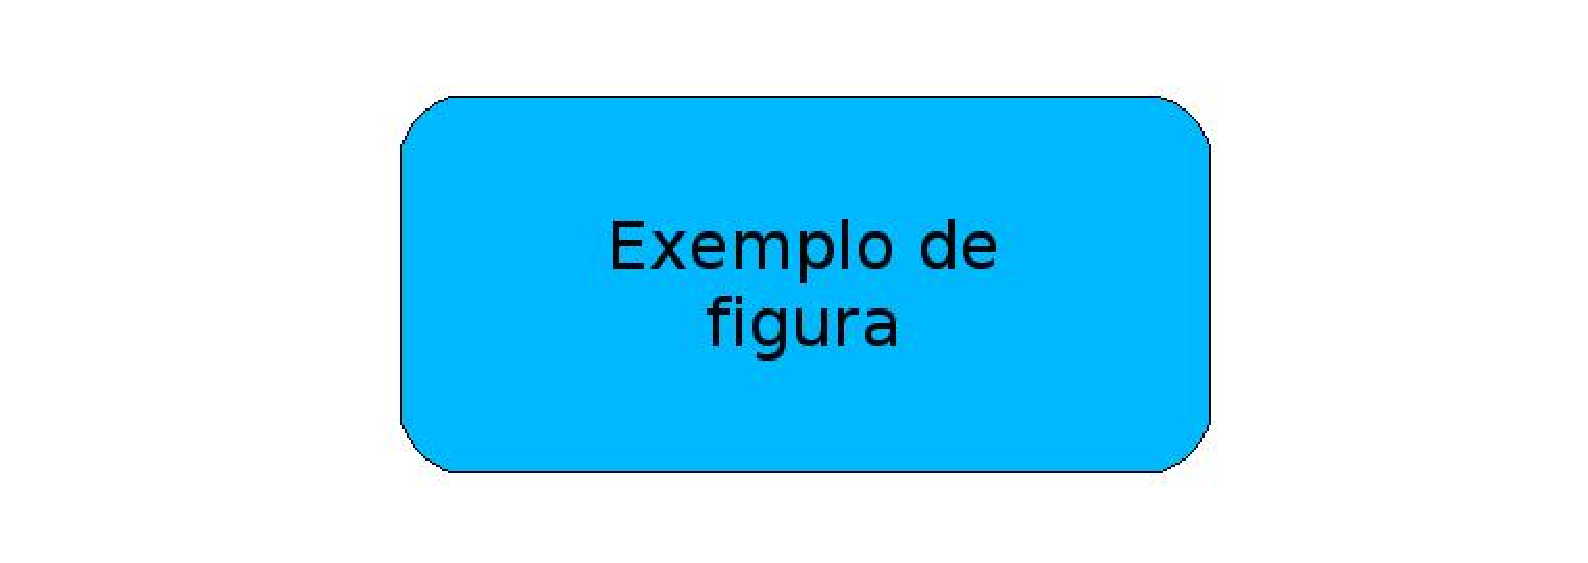
\includegraphics{figura}
  \label{fig:1}
\end{figure}

\begin{center}
  Fig. 1
\end{center}

%\newpage
%\clearpage

\begin{center}

\begin{figure}[htb]
    \begin{minipage}[b]{.46\linewidth}
%  \includegraphics[angle=0,height=7cm]{figura2}
  \vspace{5cm}
    \end{minipage}\hfill 
    \begin{minipage}[b]{.46\linewidth}
  \vspace{5cm}
   \end{minipage}
\end{figure}


% \begin{figure}[htbp]
%   \includegraphics[angle=0,width=15cm]{Figura2}
% %  \caption{ }
%   \label{fig:2}
% \end{figure}

  Fig. 2
\end{center}

\clearpage
%\newpage
\chead{\hfil 2\ / 2\hfil}


\begin{figure}[htbp]

\vspace{4cm}
%  \caption{ }
  \label{fig:3}
\end{figure}

\begin{center}
  Fig. 3
\end{center}

  
\end{center}















\end{document}



%%% Local Variables: 
%%% mode: latex
%%% TeX-master: t
%%% ispell-dictionary : brasileiro
%%% End: 
